\subsection{Bezpečnosť}
Na prvom mieste je dôležitá bezpečnosť. Riešenie, ktoré vyvíjame v tejto práci musí byť zabezpečené, aby citlivé dáta používateľov neunikli. Najmä, ak ide o password manager.

Prvým nepriateľom bezpečnosti je komplexnosť \cite{practicalcryptography}. Nehovoríme o tom, že softvér má byť malý. Aj veľké systémy vedia byť v podstate jednoduché. 

Systém je len tak bezpečný ako jeho najzraniteľnejšia časť \cite{practicalcryptography}. Preto musíme rovnako kvalitne zabezpečiť každý komponent a modul. Ak existuje trhlina v systéme, útočník ju využije. Je to jednoduchšie, ako prelomiť tú časť systému, ktorá je kvalitne zabezpečená. 

V našom riešení sa budeme pozerať na bezpečnosť jednotlivých modulov.
\begin{itemize}
    \item[-] Ako chráni Passer citlivé dáta v čase, keď aplikácia nie je používaná
    \item[-] Ako je zabezpečený prenos dát medzi jednotlivými komponentami
    \item[-] Ako sú chránené komponenty server a webstránka
\end{itemize}

\subsubsection{Passer}
Passer potrebuje chrániť dáta, ktoré sú uložené vo filesystéme iOS. Keďže nechceme, aby používateľ stratil všetky dáta po reštarte aplikácie, potrebujeme ich ukladať mimo aplikáciu. Riešením je šifrovanie. Ak zašifrujeme dáta počas ukladania do súboru, útočník ich nebude môcť rozlúštiť, aj keby sa ku nim dostal. 

Z rôznych dostupných šifrovacích algoritmov sme vybrali 
AES. Táto symetrická šifra používa len jeden kľúč. Pomocou neho šifruje, ale aj dešifruje dáta. Vzniká nám nový problém: teraz musíme chrániť aj súbory (pred poškodením, odcudzením), aj kľúč k ich zašifrovaniu. Na ukrytie kľúča sme využili architektúru, ktorú obsahujú iPhone smartfóny s technológiou Face ID alebo Touch ID: Secure Enclave.

Secure Enclave (ďalej SE) je kus hardvéru, ktorý žije spolu s telefónom pod jednou konštrukciou. Má vlastný operačný systém a funguje nezávisle od iOS. Jeho úloha je chrániť citlivé údaje telefónu, najmä kryptografické kľúče. Taktiež je používaný na bezpečnostné procedúry ako verifikácia biometrickým odtlačkom \cite{secureenclave} (Touch ID/Face ID). Má vlastný, šifrovaný firmvér, pamäť, disk a šifrovanie na úrovni hardvéru. Tento komponent využijeme na ukrytie AES kľúča. Keďže sa jedná o dve komunikačné strany, musí prebehnúť asymetrická výmena kľúčov, aby si iOS a SE mohli medzi sebou vymieňať dáta bezpečne. 

iOS nekomunikuje s SE priamo. Využíva takzvaný ,,mailbox'' (poštová schránka) systém. Aplikácia umiestni dáta a inštrukcie, čo sa má s nimi vykonať na špeciálne pamäťové miesto (mailbox). Odtiaľ si ich SE vezme, vykoná operácie a výsledok vloží späť do mailboxu, odkiaľ si ich aplikácia vezme. 
\newline
\begin{figure}[H]
  \centering
  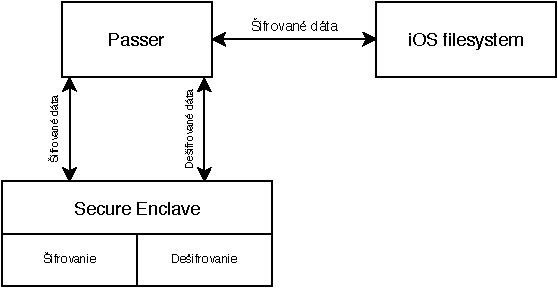
\includegraphics[width=15cm]{img/enclave.pdf}
  \caption{Interakcia Passera s iOS a Secure Enclave.}
  \label{enclave}
\end{figure}

V Secure Enclave vieme vytvárať iba 256 bitové, súkromné, elliptic curve kľúče \cite{secureenclave_appledoc}. Tieto kľúče vedia byť použité na Diffie-Hellmanovu elliptic curve (ECDH) výmenu kľúčov. A túto operáciu vieme použiť na symetrické šifrovanie. Tieto kľúče vieme vytvárať výhradne iba v SE. Nie je možné vkladať, či vyberať už existujúce kľúče. Nemožnosť týchto úkonov je základom celej bezpečnosti SE. 

Vytvorenie súkromného, elliptic curve kľúča vyzerá v jazyku Swift nasledovne:

\begin{center}
    \texttt{let privateKey = SecKeyCreateRandomKey(attributes as CFDictionary, \&error)}
\end{center}

\noindent Kde \texttt{attributes} je \texttt{dictionary} atribútov súkromného kľúča, kde definujeme jeho vlastnosti (256-bit elliptic curve a pod.). Tento kľúč vytvárame priamo v Secure Enclave. Do premennej \texttt{privateKey} ide iba referencia skutočného kľúča \cite{secureenclave_appledoc}, takže zdroj je uchovaný v SE. Preto nie je možné získať z \texttt{privateKey} jeho dáta, takže tu je bezpečnosť zachovaná. 

Z \texttt{privateKey} vieme získať verejný kľúč a to nasledovne: 

\begin{center}
    \texttt{let publicKey = SecKeyCopyPublicKey(privateKey!)}
\end{center}

\noindent Máme vytvorený súkromný aj verejný kľúč, ktorý patrí Secure Enclave. Môžeme začať so šifrovaním.

Symetrické šifrovanie prebieha podľa algoritmu ECIES \cite{ecies}. V kryptografii sa komunikácia medzi dvoma stranami demonštruje ako komunikácia medzi Alicou a Bobom. Bob bude v našom prípade Secure Enclave, Alica bude Passer. Teda:
\begin{itemize}
    \item[-] Bob vlastní súkromný kľúč $x$ a z neho vytvorí verejný kľúč $g^{x}$. 
    \item[-] Alica získa Bobov verejný kľúč $g^{x}$.
    \item[-] Alica vygeneruje súkromný, efemérfny kľúč $y$ a z neho verejný, efemérfny kľúč $g^{y}$.
    \item[-] Alica vypočíta symetrický kľúč $k$ pomocou key derivation function: $k = KDF(g^{xy})$.
    \item[-] Alica získa šifrovaný text $c$ zo správy m použitím symetrického kľúča $k$ a algoritmu $AES$ nasledovne: $c = AES(k;m)$.
    \item[-] Alica pošle šifrovanú správu spolu s efemérfnym kľúčom Bobovi. 
    \item[-] Bob extrahuje z $c$ efemérfny verejný kľúč.
    \item[-] Bob vypočíta symetrický kľúč k pomocou key derivation function: $k=KDF(g^{xy})$
    \item[-] Bobov kľúč $k$ je rovnaký, ako Alicin pri šifrovaní.
    \item[-] Bob dešifruje správu $c$ a získa otvorený text: $m = AES(k;c)$.
\end{itemize}

\noindent Zobrazme si tento proces vizuálne. Pri šifrovaní
\begin{figure}[H]
  \centering
  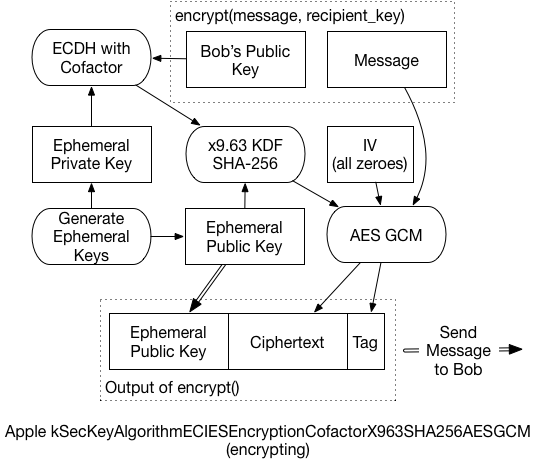
\includegraphics[width=15cm]{img/ecies-arch-encrypt.png}
  \caption{Proces šifrovania podľa algoritmu ECIES.}
  \label{SEencr}
\end{figure}

\noindent vznikajú efemerálne kľúče. Efemerálny súkromný kľúč spolu s verejným kľúčom patriacim Secure Enclave na základe ECDH vytvoria takzvaný ,,shared secret''. Ten je pomocou KDF zmenený na symetrický kľúč. Kľúč vchádza do AES spolu so správou a inicializačným vektorom. Výsledok je zašifrovaný text spojený s efemerálnym verejným kľúčom a tagom. Tento ,,balík'' je odoslaný do SE. 
\begin{figure}[H]
  \centering
  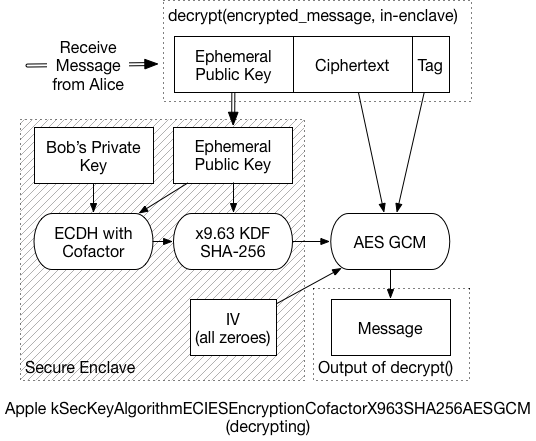
\includegraphics[width=15cm]{img/ecies-arch-decrypt.png}
  \caption{Proces dešifrovania podľa algoritmu ECIES.}
  \label{SEdecr}
\end{figure}

SE spracuje to, čo prišlo. Extrahuje efemerálny verejný kľúč. Použije svoj súkromný kľúč a a efemerálny verejný kľúč na získanie verejného tajomstva. Pomocou KDF získa symetrický kľúč. Ten spolu s inicializačným vektorom, šifrovaným textom a tagom vstupuje do AES. Algoritmus dešifruje text na pôvodnú správu. Jediné čo SE vráti do mailboxu je táto dešifrovaná správa.

V skratke: pri šifrovaní používame verejný kľúč SE, pri dešifrovaní zase súkromný kľúč SE. Efemerálne kľúče sa generujú kvôli dohode o výmene kľúčov (ECDH). 

V zdrojovom kóde Passera existuje trieda \texttt{Vault}. V nej sú všetky položky používateľa počas behu programu: teda, v plaintexte. Po pridaní alebo vymazaní položky sa vo \texttt{Vault} zavolá metóda \texttt{vaultUpdate()}, ktorá vykonáva operácie s dátami. Najprv aktualizuje polia Passer položiek. Potom ich serializuje do JSON štruktúry. Potom túto štruktúru zašifruje pomocou \texttt{vaultEncrypt()}. Táto metóda vracia 
\begin{center}
    \texttt{return SecKeyCreateEncryptedData(publicKey!, algorithm, dataToEncrypt as CFData, \&error) as Data?,}
\end{center}
\begin{sloppypar}
    \noindent čo je zašifrovaný text. Na šifrovanie je použitá vstavaná metóda Swiftu \texttt{SecKeyCreateEncryptedData()}, ktorá ako vstup očakáva verejný kľúč SE, zvolený šifrovaný algoritmus (v našom prípade AES), nezašifrovanú správu (JSON štruktúra s Passer položkami) a smerník na objekt riadenia chýb, ktorý kontroluje chyby a oznámi ich do konzoly v prípade zlyhania.
\end{sloppypar}

Pri najbližšom spustení aplikácie je najprv od používateľa vyžiadaná biometrická autentizácia. Po úspešnom verifikovaní sa zavolá metóda \texttt{vaultDecrypt()}, ktorá dešifruje dáta a vráti ich: 
\begin{center}
    \texttt{return SecKeyCreateDecryptedData(privateKey!, algorithm, dataToDecrypt! as CFData, \&error) as Data?}
\end{center}
\begin{sloppypar}
    \noindent Metóda \texttt{SecKeyCreateDecryptedData()} očakáva súkromný kľúč SE, zvolený šifrovaný algoritmus (v našom prípade AES), zašifrovanú správu a smerník na objekt riadenia chýb.
\end{sloppypar}

Dáta sú dešifrované. JSON objekt vieme deserializovať a naplniť z neho \texttt{Vault}. Úvodná inicializácia je hotová. Používateľovi sa zobrazí úvodná obrazovka a vidí svoje Passer položky. 

Pri úvodnej biometrickej autentizácii nešlo o šifrovanie/dešifrovanie/výmenu kľúčov. Je to len podmienka k tomu, aby mohlo dešifrovanie vôbec začať. Ak používateľ nemá žiadne položky, tento krok je preskočený. Je zbytočné autentizovať vstup do niečoho, kde nič nie je.

\subsubsection{Server a webstránka}
Server a webstránka sú komponenty, ktoré sú neustále v sieti internet, takže sú kedykoľvek dosiahnuteľné. No najmä, dostať k nim dáta znamená prenášať ich po sieti. Preto je dôležité, aby bol protokol HTTP zabezpečný a Eva\footnote{pri spomínanom Bobovi a Alici je Eva chápaná ako útočník, ktorý chce spojenie narušiť alebo čerpať z neho citlivé informácie} nevedela kanál čítať. Z toho dôvodu sú oba komponenty zabezpečené HTTPS protokolom, ktorý zaobaľuje vrstvu HTTP do TLS vrstvy. Tá šifruje informácie, ktoré cestujú z Passera na server, zo servera na webstránku, z webstránky na server.

Server nemá žiadne dáta vo filesystéme. Teda, narozdiel od Passera nemusíme riešiť problematiku ukladania a výmeny kľúčov. Jediné dáta, ktoré server uchováva sú v cache. Lenže tie musia byť v plaintexte, pretože sa používajú v reálnom čase pri rôznych operáciách.

Webstránka je na tom podobne. Prijaté dáta od servera po úspešnej verifikácii používateľom sú rovnako v plaintexte, pretože ich potrebujeme zobraziť na obrazovke. Taktiež musí byť používateľ schopný ich skopírovať. Keby skopíroval šifrovaný text, používanie jeho údajov by bolo zbytočné, nakoľko by boli šifrované.

Aby sme po sebe nezanechali stopy, vždy po získaní dát od servera vyčistíme local storage. Inak by boli dáta dohľadateľné v každej session, pokiaľ je otvorený prehliadač na cudzom zariadení.